\documentclass{report}
\usepackage{fullpage}
\usepackage{graphicx}
\usepackage[procnames]{listings}
\usepackage{amsmath}

\renewcommand{\baselinestretch}{2}
\author{Mukesh P., Aniket Patel \\ Project mentor: Amiraj Dhawan} 

\title{Depth based room mapping using Kinect}
\begin{document}
\maketitle
\tableofcontents


\chapter{Abstract}
In this project, an indoor path planning algorithm is proposed for autonomously detecting and exiting a door. Complex situation in indoor
environment may lead to serious problem with analysis of data to process corners and edges of doors. For this reason, a Kinect is used.
Kinect can give depth information of an image. This depth information from Kinect is processed to detect edges and corners of a door and using serial
communication, the robot is made to exit the room. Experiments on different indoor scenarios have been performed
to verify the efficiency of algorithm.
\chapter{Objective of the work}
The aim of this project is to use the depth sensing to create a depth map of a room using Kinect sensor. The robot is used for movement and the 
Kinect to create a depth map of the room. The final goal is to exit the room from the only single door depending on the depth map created. \\ \\

\begin{tabular}{ | c | c | c |}
	\hline\hline
	\bf Sr.No & \bf Tasks & \bf Deadline \\ 
	\hline
	1.) & Learning Fire Bird V programming, Kinect API & 5 days \\
	\hline
	2.) & Develop code for Fire Bird V movement & 3 days \\
	\hline
	3.) & Creation of Depth Map for the room using Kinect & 5 days \\
	\hline
	4.) & Decision making about exiting the room based on depth map & 12 days\\
	\hline
	5.) & Testing/Documentation (Usage Manual, Documented Code) & 5 days
	\\ \hline

\end{tabular} \\

\chapter{Completion}

All tasks have been completed. Robot exits the door through the door present in the room in about 80\% of cases.
The following work has been done in each task.

\section{Task 1- Learning FireBird V and Kinect API}
\begin{itemize}
\item Installed the following libraries:
\begin{itemize}
 \item \textbf{freenect}: This library contains necessary modules for installing Kinect. It provides sample 
			  programs which can be used to test the functionality of Kinect.
 \item \textbf{python wrapper for freenect}: This library is used for reading data from Kinect in python.
 \item \textbf{opencv}: This library provides various modules which are used for processing an image. The data retrieved from
			Kinect has a lot of noise. This image can be converted into a grayscale image and modules of opencv are applied to remove noise.
 \item \textbf{numpy}: numpy provides an easier way to use arrays in python.
 \item \textbf{matplotlib}: In our project, matplotlib is used to create a Gaussian distribution curve and calculate probabilities.
\end{itemize}

\item Learned various Kinect modules to perform the following operations:
\begin{itemize}
 \item Retrieve a depth map from Kinect. (3.3)
 \item Control the motor of the Kinect.
 \item Retrive image from the RGB camera of Kinect.
 \item Control the LED's present on the device
\end{itemize}

\end{itemize}

\section{Task 2 - Develop a code for FireBird movement}



The robot will move forward till it can deduce that it is at a sufficient distance from a wall. 
This will be decided by taking the mean of pixels in a particular space. After this, the robot
will move along the wall and detect doors in the given space. It will map and keep a record of all the objects that look 
like a door. One can never be sure whether a rectangular object detected is a door or not. Hence, 
every such object will be associated with a probability. If this probability is above a threshold 
value, then the robot will decide that the obstacle detected is a door and will exit through it. 
If not, then it will scan the rest of the arena and keep storing information about obstacle, their 
position and probabilities and after scanning the room, it will choose the door having highest
probability. \\
Two types of movements have been defined for robot traversal.

1. Regular movement:

This algorithm is used when the robot is trying to detect a door. In this algorithm, the image is divided into 8 frames. Suppose the frames are numbered consecutively from left to right. If a obstacle appears in the first frame, the robot will take a soft turn. As the obstacle starts getting closer to the middle area, the velocity is increased so that the robot takes a hard turn. There may exist two cases:
\\ \\ \\ \\ \\ \\
Case 1: Obstacle which lie beyond 40cm:

In this case, the obstacle lies within Kinect's detection range. Hence, the movement of the robot looks something like this:

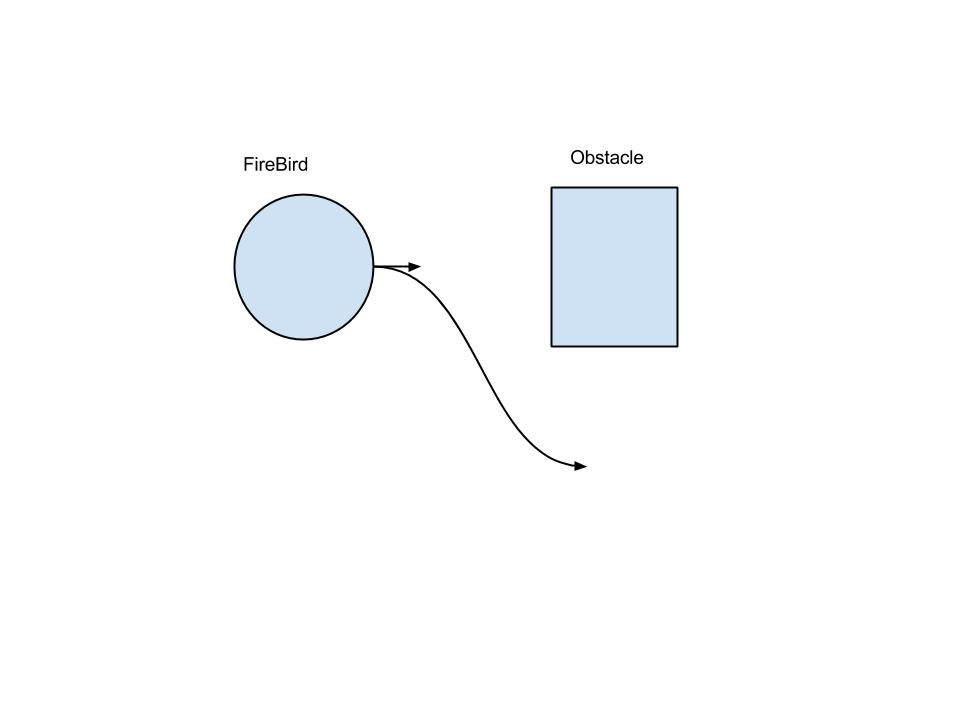
\includegraphics[width = 20CM]{Case_1.jpg}
\\ \\ \\ \\ \\
Case 2: Obstacle which lie between 0 - 40cm:

In this case, the obstacle does not lie within the Kinect's detection range. 
The obstacle is detected using GP2D12 Sharp sensors. The movement of the robot would look something like this:
\begin{flushleft}
 

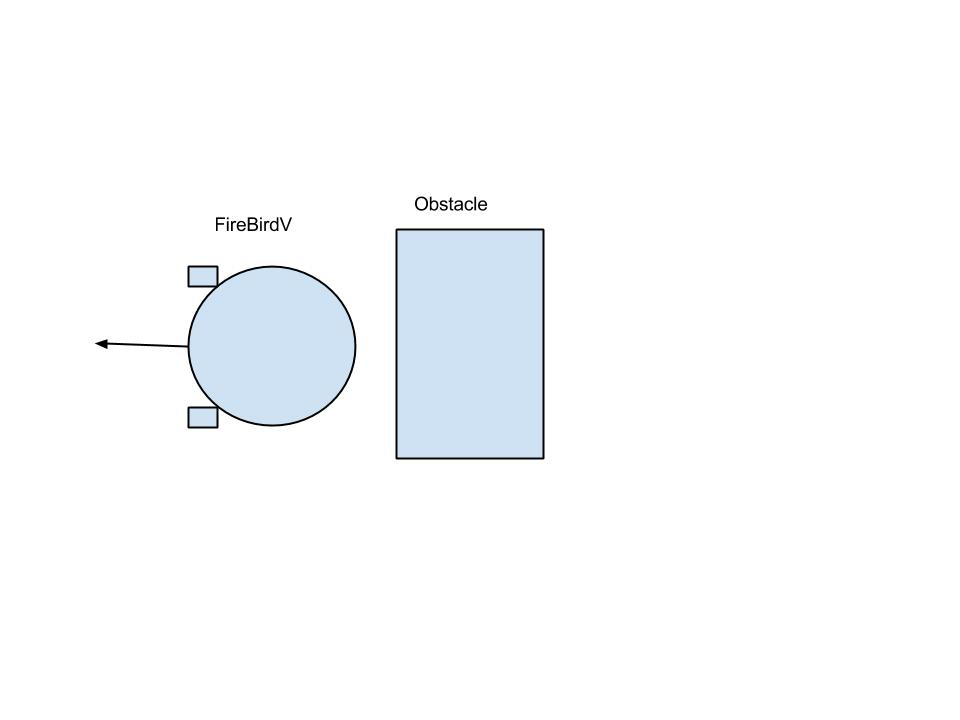
\includegraphics[width = 20CM]{Case_2.jpg}

\end{flushleft}

2. Doorway Movement:
This algorithm is used when a door is detected. After a door is detected, 
the image is divided into three vertical frames (left, middle and right frame). 
if there is sufficient space in middle frame, then the robot moves forward. Else, 
depth in right and left areas are compared to decide whether a left turn should be taken or a right turn.

\section{Task 3 - Creation of a depth map of room using Kinect}
Under this task, a depth map of the environment was obtained from Kinect. A depth map is an image which contains information about
depth in every pixel. So, when such a raw feed is converted into a grayscale image, the objects that are closer to the Kinect appears darker
than the objects away from Kinect. Example: \\

The original image: \\
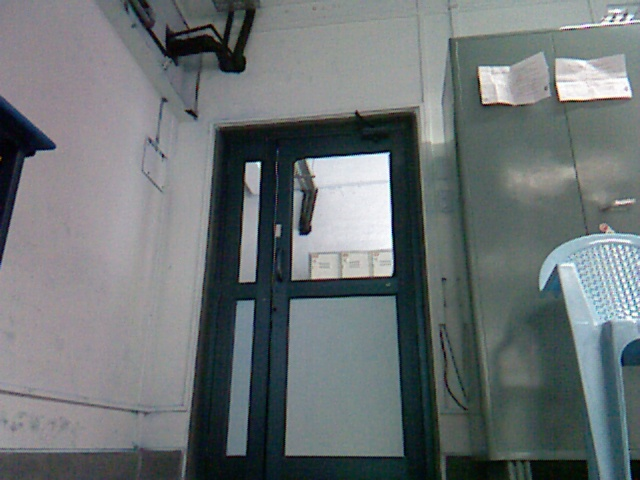
\includegraphics[width = 10cm]{reference.jpg} \\
Depth Map:\\
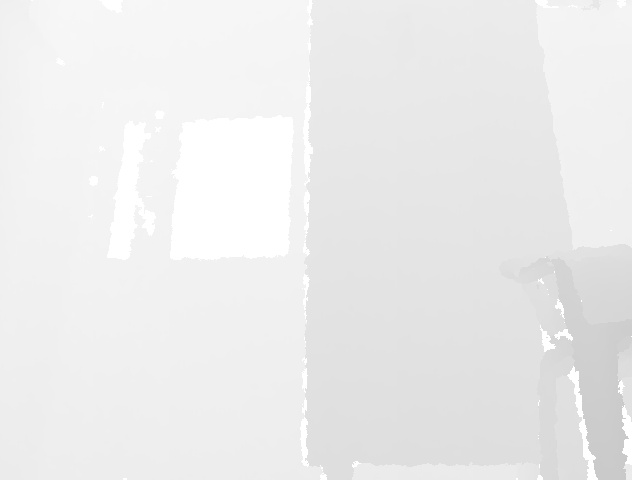
\includegraphics[width = 10cm]{feed.jpg} \\
The depth map of the environment can be retrieved from Kinect in python using: \\
\begin{lstlisting}
depth = freenect.sync_get_depth(format=freenect.DEPTH_11BIT)
\end{lstlisting}
After retrieving the depth map, bilateral filter is applied on the image obtained to reduce noise and still pertain edges. After
applying bilateral filter, the image now becomes : \\
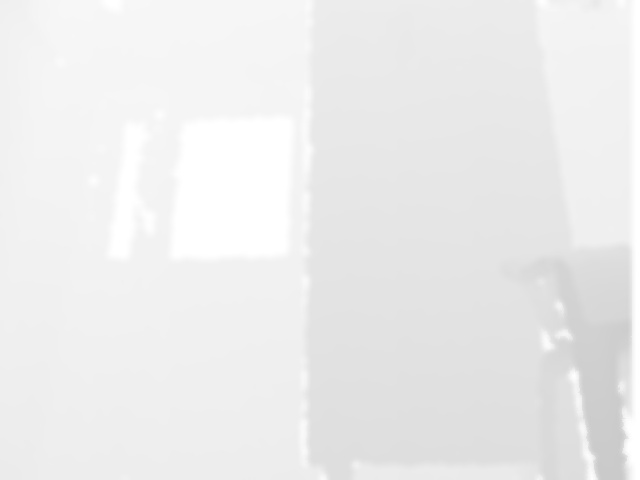
\includegraphics[width = 10cm]{bilat.jpg}

After further research, It was realized that it is beneficial to use a different format for the feed which returns depth of each pixel 
in mm. This feed can be retrieved using: \\
\begin{lstlisting}
depth = freenect.sync_get_depth(format=freenect.DEPTH_MM)
\end{lstlisting}

The depth feed is a numpy array and contains values ranging from 0 to 8000mm: 0 represents unknown distance. Unknown distance may be 
obtained due to any reflective surface like mirrors or glasses. These values can be fit into the range 0-255 by converting it 
into grayscale image and ignoring few lower bits. Results of ignoring different amounts of lower bits are shown below. \pagebreak
\\
Image after ignoring lower 4 bits: \\
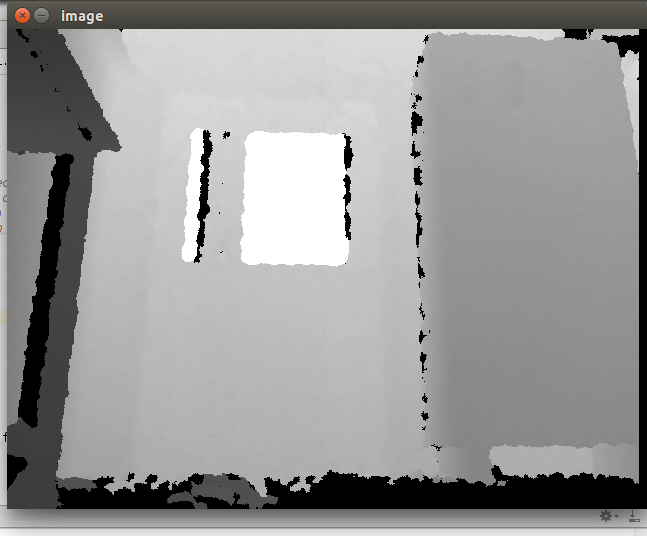
\includegraphics[width = 10cm]{d_4bit.png} \\
Image after ignoring lower 5 bits: \\
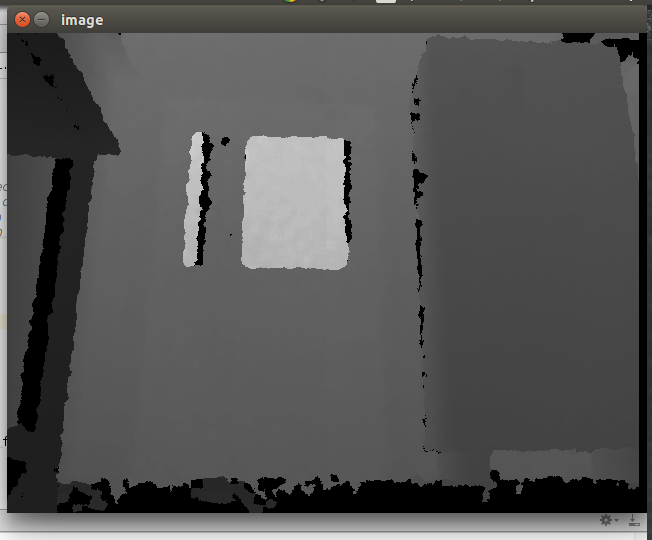
\includegraphics[width = 10cm]{d_5bit.png} \\
\pagebreak

Image after ignoring lower 3 bits and clipping \\
\begin{center}
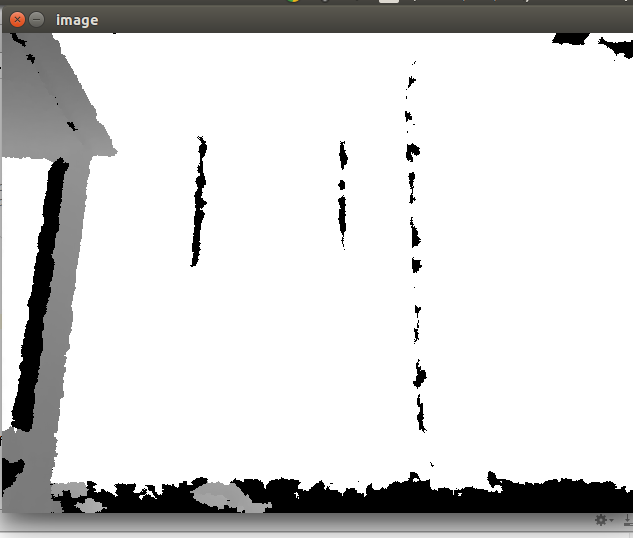
\includegraphics[width = 10cm]{d_3bit.png} \\
\end{center}

This feed is filtered using the following method:
This algorithm is similar to the algorithm used for median blur. A kernel element is taken and the mean of the depth array in the
kernel element is calculated. The pixels where depth cannot be calculated contains zero value. Such noise pixels are replaced
with the mean value calculated before using simple masking techniques. The result of this filter on an image is shown below.\\
\pagebreak

Noisy image: \\ 
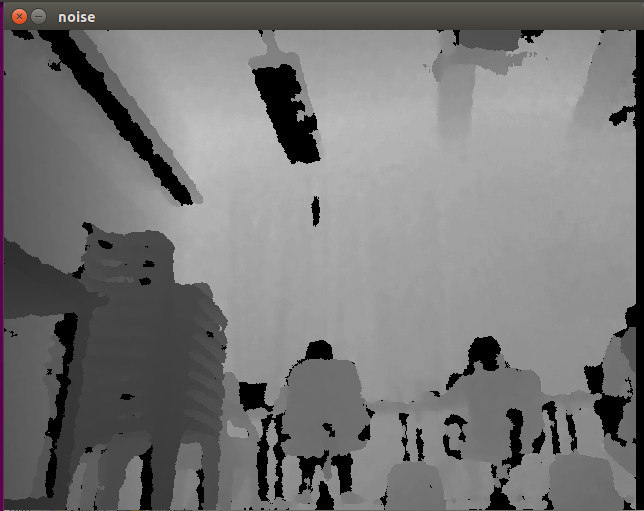
\includegraphics[width = 10cm]{Noise.png} \\
After applying filter: \\
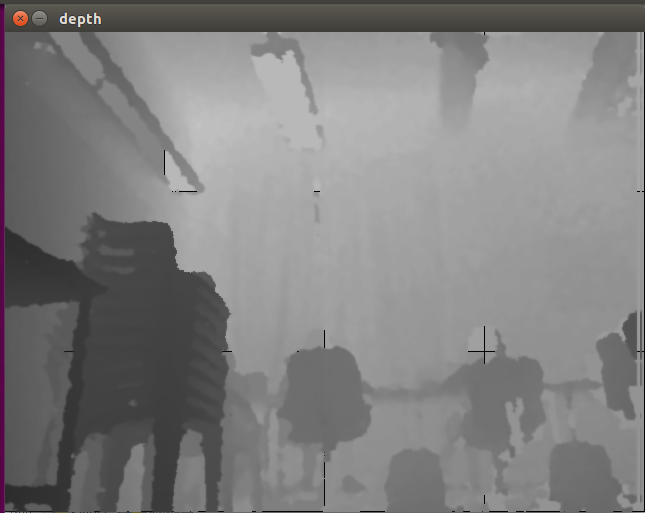
\includegraphics[width = 10cm]{Noiseless.png} \\

\section{Task - 4: Decison making about exiting the room based on depth map}

In this project, 4 basic tests are used to determine whether an obstacle having left and right edges is a door or not.

\textbf{Test 1: Depth analysis to determine edges} \\

First, the image feed is retrieved from Kinect and noise is removed using steps mentioned in previous task. After this,
 A copy of this image is made and every row element is shifted by one column. The difference between both the arrays is calculated and stored in another variable. 
 Every element of this array is multiplied by 255. Hence, we have a resultant image which contains 
 the edges of obstacles. These edges can be retrieved by thresholding and taking contours of the 
 resultatnt image. Note: Right or left edge depends on which array is subtracted from which array. 
 Subtracting the final array from the initial array will give all the left vertical edges of obstacles. 
 All contours in this resultant image are calculated. Every contour having area less than a threshold value are ignored. After filtering objects with respect to 
 height, the resultant image is obtained: \\

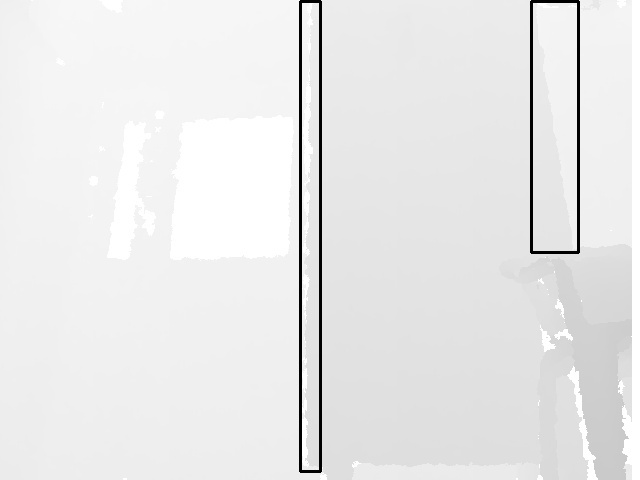
\includegraphics[width = 10cm]{result.jpg} \\

The co-ordinates for contours of bigger obstacles are processed again. If a left edge (outgoing) 
appears before a right edge (incoming edge), then the object can be considered as a door. If a right 
edge appears  before the left edge, then the obstacle is something different than a door, maybe a
cupboard.

\textbf{Test 2: Height analysis:} \\
The height of obstacles are calculated using basic trigonometric operation.

First, the edges of the obstacle are segregated using methods from previous test. 
A bounded rectangle is formed around this contour. Now, the depth of the topmost point and the nearest 
point are noted. These values must be the base and hypotenuse of a triangle as shown: \\

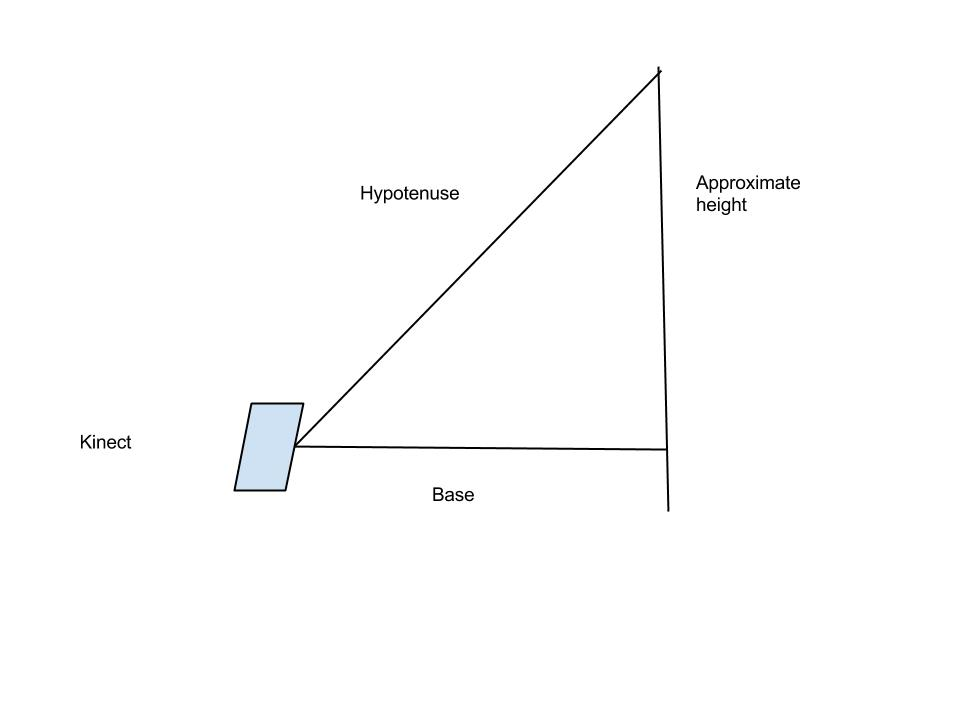
\includegraphics[width = 10cm]{pythagoras.jpg}

This height is compared with the standard height of a door. The standard height of a door is 2000mm. 
The difference between calculated height and actual height gives the error in height. Using this height, 
a probability value can be estimated which will reflect how much a particular obstacle passes this test. 
The probability is calculated using a Gaussian Distribution curve. \\
\pagebreak

Gaussian distribution is a very common continuous probability distribution. The normal distribution is sometimes informally called the bell curve.
A bell curve appears as shown:\\

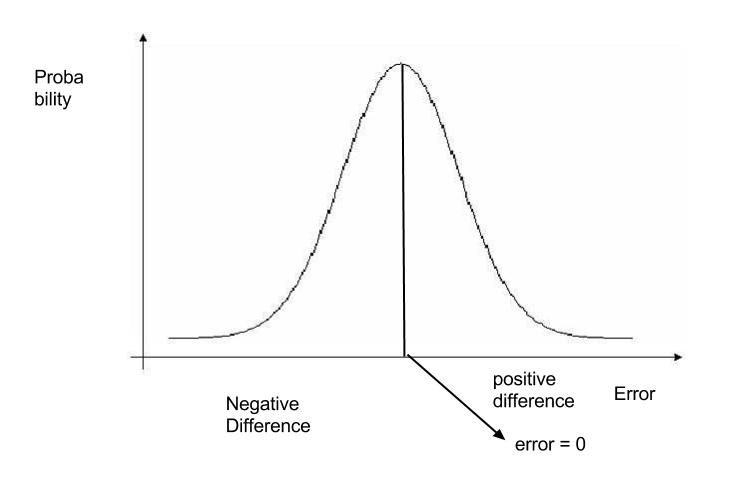
\includegraphics[width = 10cm]{Gaussian.jpg} \\
The probability density of the normal distribution is:
\begin{equation}
f(x|\mu,\sigma) = \frac{1}{\sigma\sqrt{2\pi}}e^{-(\frac{(x-\mu)^2}{2\sigma^2}}
\end{equation} \\
Here, $\mu$ is the mean or expectation of the distribution (and also its median and mode)
The parameter $\sigma$ is its standard deviation with its variance then $\sigma^2$. A random variable with a Gaussian distribution 
is said to be normally distributed and is called a normal deviate. \\
In the tests performed in this projects, the probability depends on the value 'x - $\mu$'. 'x' is the  value obtained by depth calculations.This difference determines the probability
whether the obstacle in front of camera is a door or not. When the difference is 0, maximum probability i.e. 1 is obtained. Distribution
curve behaves in a similar way for both negative and positive difference. Initially, for a certain value, the rate of change or the rate
of fall of probability is low. As the difference increases, the rate of change increases exponentially. For the purpose of detection of doors, where
a deviation from ideal value is always expected, this curve is instrumental. \\
\pagebreak

\textbf{3: Width analysis:} \\

This test is similar to the previous test. The width of the door is calculated as shown: \\

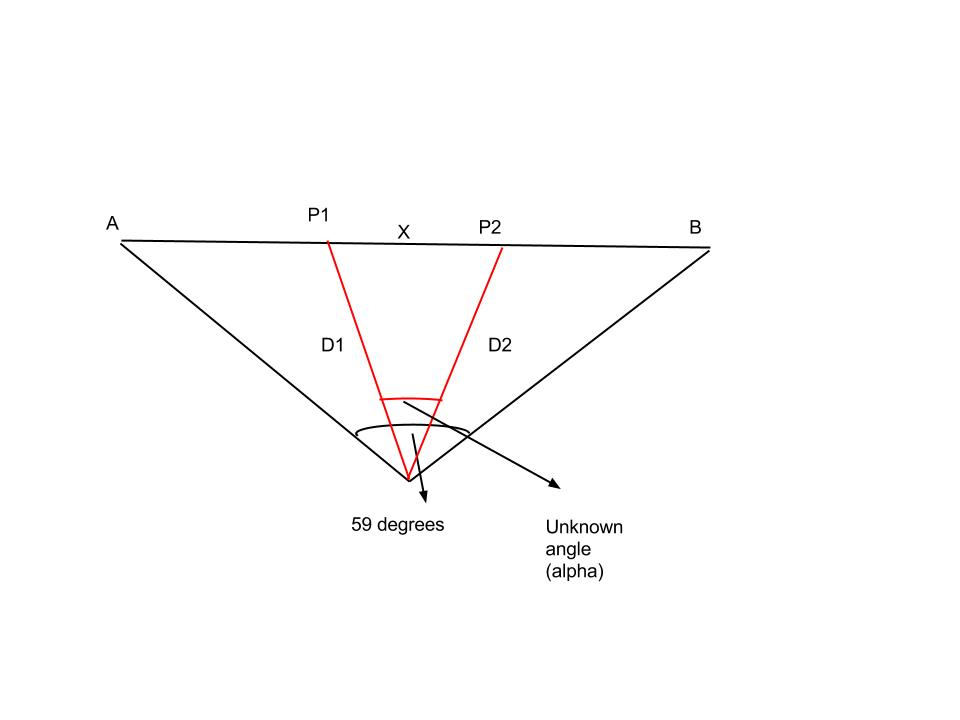
\includegraphics[width = 10cm]{Cosine.jpg}

The field of view of Kinect covers an angle of 57 degrees. The total pixel count in horizontal direction is 640. Suppose we need the width x. We first calculate the ratio at which the pixels are divide. This will be equal to:
\begin{equation}
P1(x) - \frac{P2(x)}{640}
\end{equation}

Now, the angle alpha will also divide the total angle in equivalent proportions. Hence, 
\begin{equation}
\alpha = P1(x) - \frac{P2(x)} {640} * 57
\end{equation}

Now, once we know the sides of a triangle and angle between them, the distance x can be calculated by using cosine rule:
\begin{equation}
X = D1^2 + D2^2 - 2*D1*D2*\cos{\alpha}
\end{equation}
\pagebreak

\textbf{4: Horizontal edge test:} \\

This test can only be applied when a horizontal edge(or the upper edge) of the door is detected. In this test, the depth map numpy array is shifted to a value equal to five times the maximum width of frame viz 640 pixels. This will cause every element to shift by multiple columns. Hence, the difference of original array from this array will give areas where there's a difference in depth. Segregating these areas, contours can be identified where an horizontal edge lies. These edges can again be separated based on whether the edge is an outgoing (negative difference) or a incoming (positive difference) edge.

In this test, a horizontal edge is identified which lies between two vertical edges. The centroid of this horizontal edge is calculated. This must approximately lie at the centre of the centroid of edges. The difference between these two values is the required error. Probability is calculated based on this error.

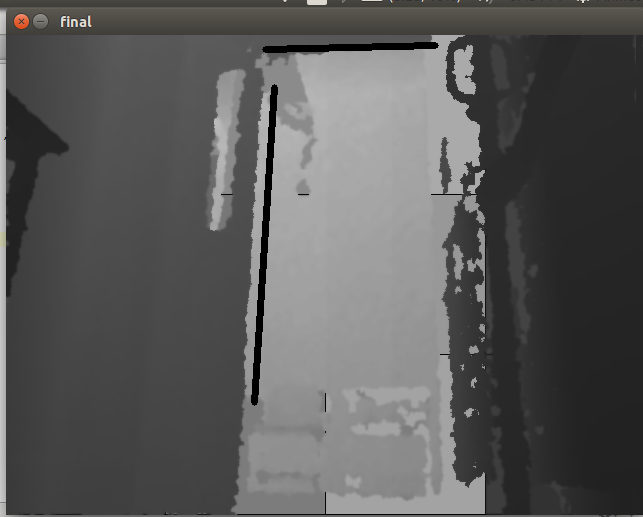
\includegraphics[width = 10cm]{horizontal.png}

\chapter{Result and discussion:} 
The end product consists of a Kinect mounted on FireBird V. It can never be ascertained that the obstacle present in front of
the robot is a door or not. For this reason, every such obstacle which is detected as a door is associated with a confidence
level. This confidence value is a result of weighted sum of the tests. It is used as the basis for determining whether the robot
should exit the door or not.

\section{Weighing of probabilities:}

This project contains four tests as mentioned in section 3. The first test only detects presence of a door like object. A probability
value cannot be obtained from the first test. The remaining three tests return a probability value. \\
Through experiments, it was found that
if the robot is close to the door, a horizontal edge may not be detected. For this reason, the weight of the fourth test is lower than the weight of second and third test.
Also, by experiments, it was observed that the calculations of height are more accurate than the width calculation. For this reason, the weight of
second test is slightly greater than that of third test.\\
Weights given to  different tests:\\
\pagebreak

Height analysis test: 50 \% \\
Width analysis test: 40 \%
Horizontal edge analysis test: 10 \% \\
The end product has been tested on various environments. Few of the environments along with the confidence levels are shown as follows:
\begin{itemize}
 \item SIC304. Average confidence level - 85\% \\
 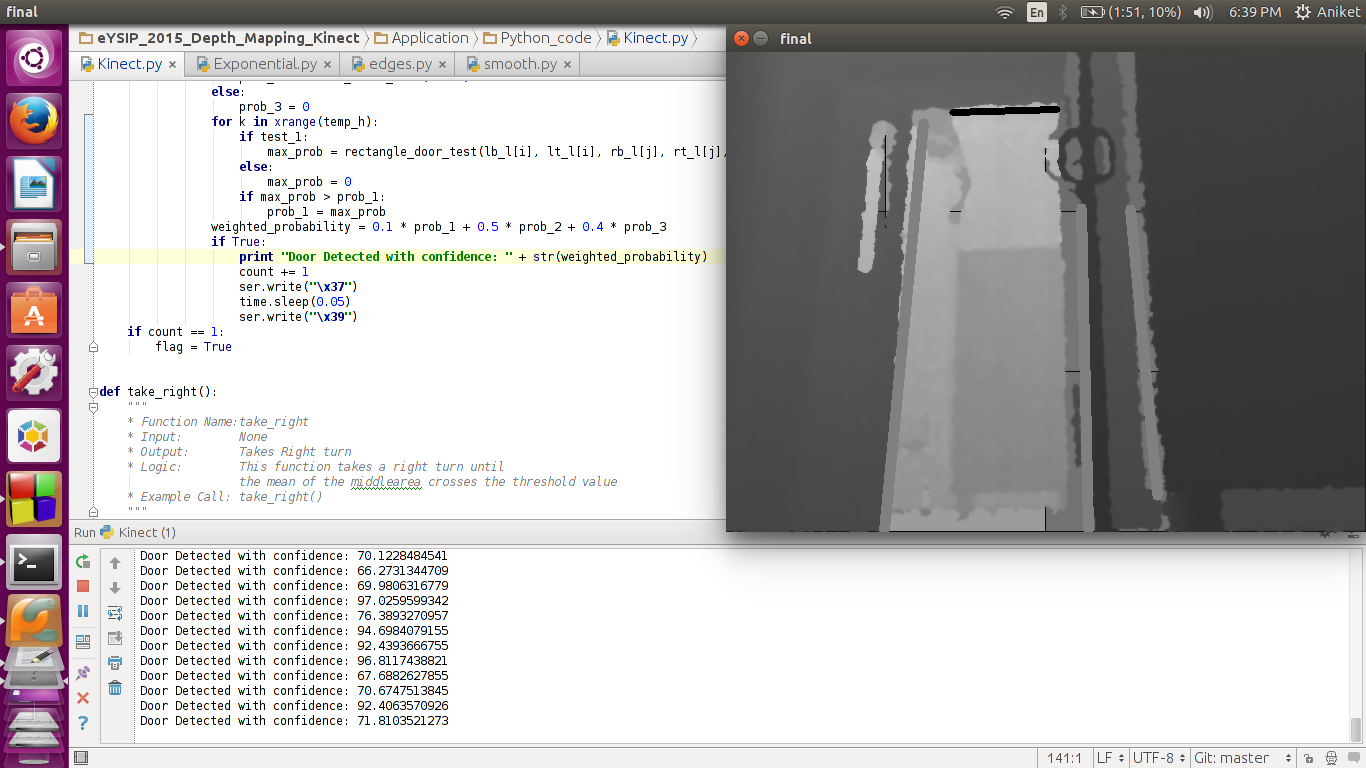
\includegraphics[width = 15cm]{confidence_304.png} \\ \\ \\ \\ \\ \\ \\ \\ \\ \\ \\ \\ \\
 \item SIC204. Average confidence level - 86\% \\ 
 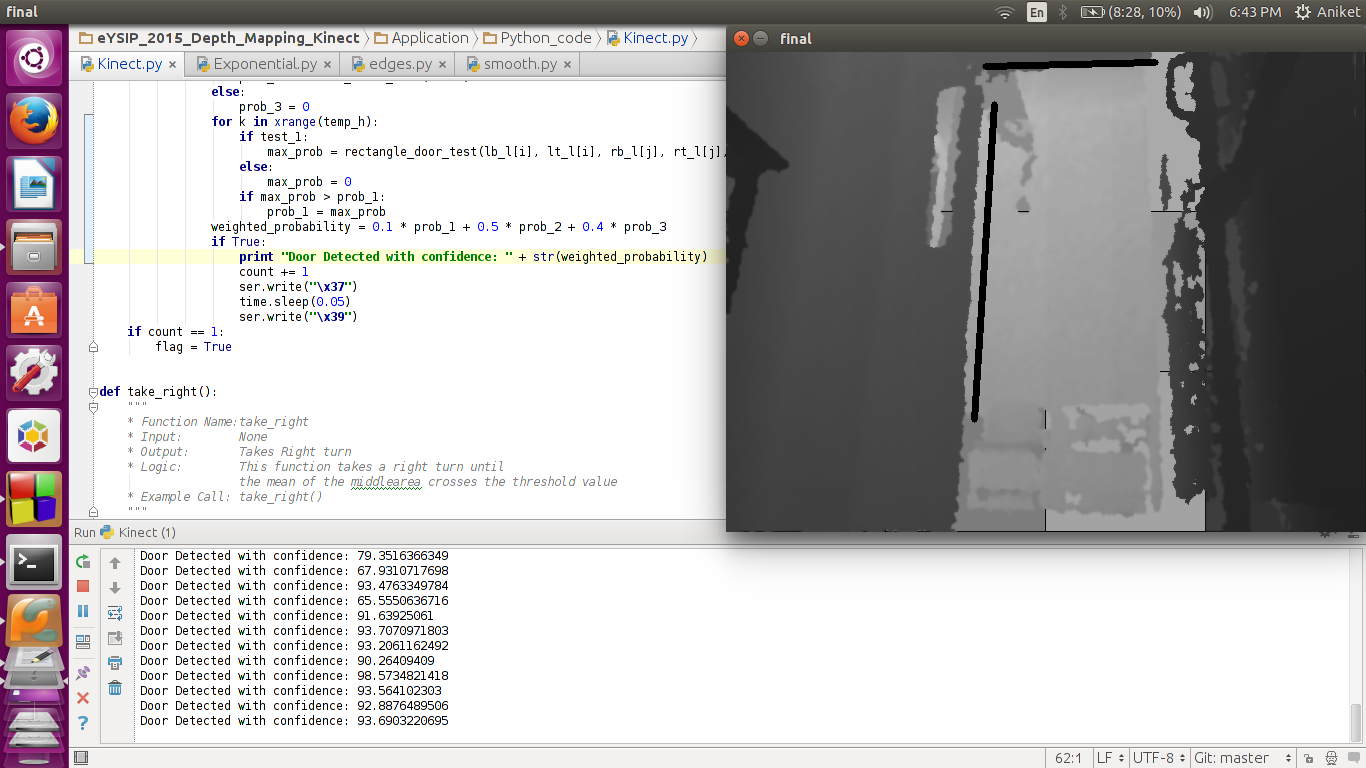
\includegraphics[width = 15cm]{confidence_204.png} \\
 \item Elevator door. Average confidence level - 70\% \\
 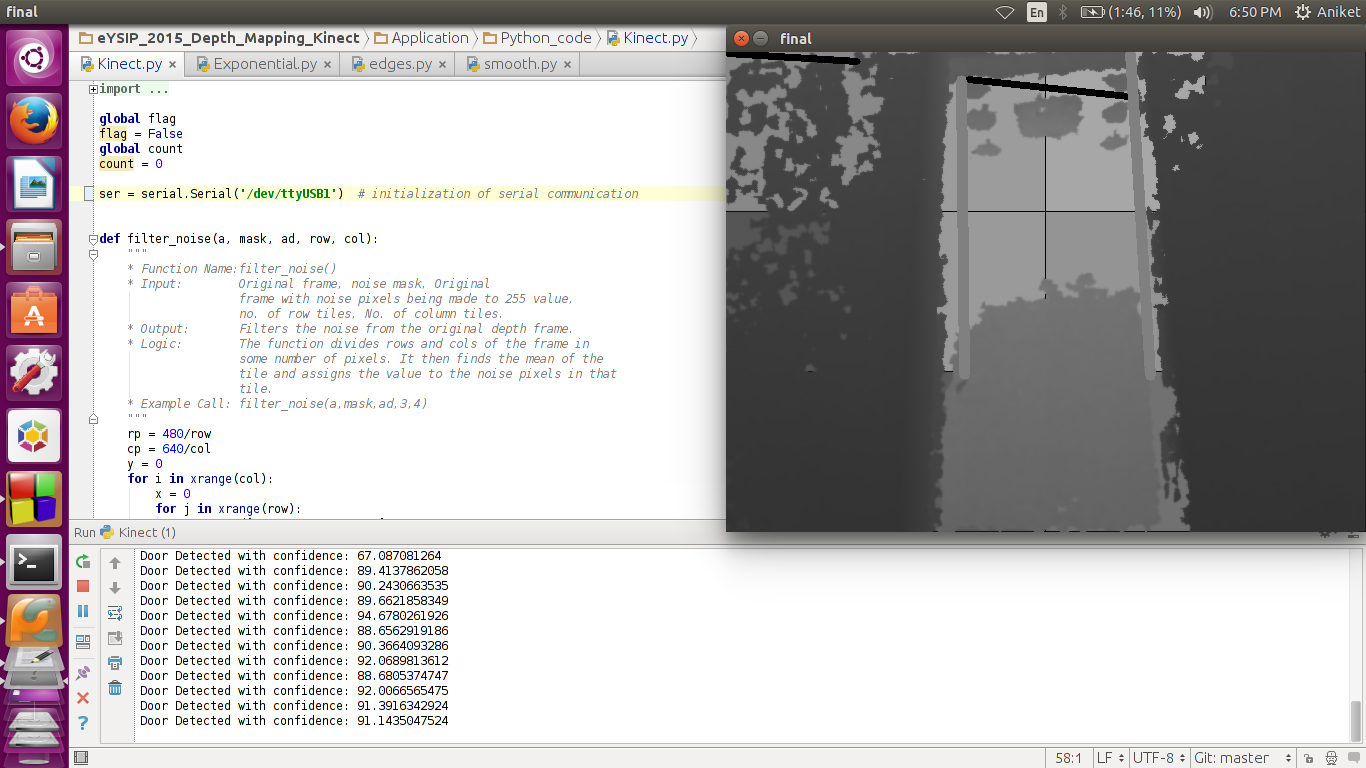
\includegraphics[width = 15cm]{lift.png} \\
 \item ERTS labs. Average confidence level - 65 \% \\
 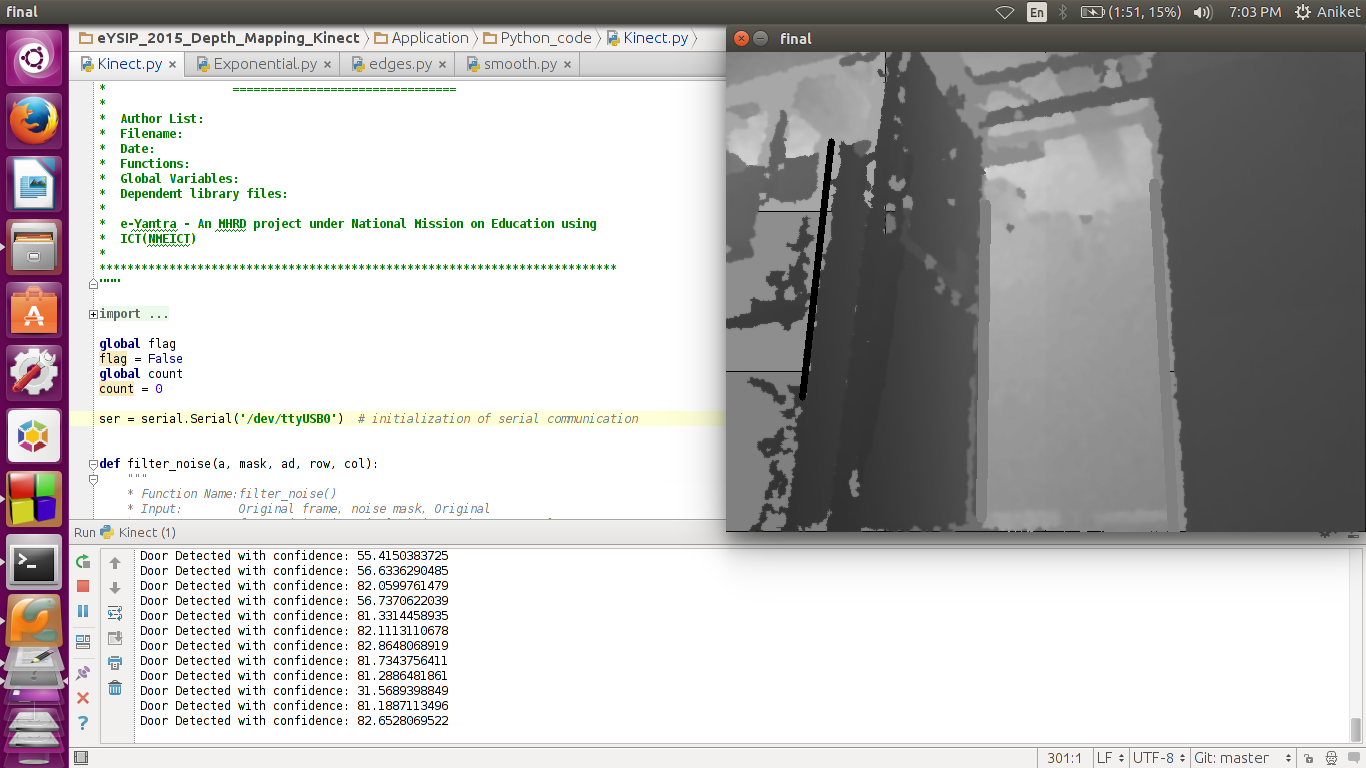
\includegraphics[width = 15cm]{erts_lab_confidence.png} \\

\end{itemize}


\chapter{Issues}
\begin{enumerate}
 \item Loose connection of wires: Sometimes, the program stopped due to loose connection of serial cable. This was fixed by using
 XBEE communication instead of serial cable.
 \item The method used for calculation of width is not accurate. Sometimes, it may give values very different from the actual value.
\end{enumerate}



\chapter{Future Work}

\begin{enumerate}
 \item \textbf{Floor planning}: Currently, floor planning has not been considered. It is assumed that the surface on which the
 robot moves is flat. This might not always be the case. Floor planning can be done in order to detect surfaces over which robot
 cannot move. This will also add as a feature of door. A door must start from ground. Hence, another test can be developed
 which will utilize this feature.
 
 \item \textbf{Using different robots}: The whole system can be ported to FireBird VI which will be able to handle heavier objects more efficiently.
\end{enumerate}

\chapter{References}
\begin{enumerate}
 \item $http://ieeexplore.ieee.org/stamp/stamp.jsp?arnumber=6926245$
 \item $http://docs.opencv.org/3.0-beta/doc/py\_tutorials/py_tutorials.html$
 \item http://openkinect.org/wiki/Documentation
 \item $http://ieeexplore.ieee.org/stamp/stamp.jsp?tp=\&arnumber=6573398\&tag=1$
 \item $http://campar.in.tum.de/pub/hinterstoisser2011linemod/hinterstoisser2011linemod.pdf$
 \item $http://www-home.htwg-konstanz.de/~bittel/Publikationen/icaart_doordetection_2010.pdf$
 \item $http://research.ijcaonline.org/volume86/number8/pxc3893182.pdf$
 \item $http://www.intel.com/content/dam/www/public/us/en/documents/guides/bkm-installing-ubunto-os-on-de2i-150-board-guide.pdf$
 \item $https://github.com/amiller/libfreenect-goodies$
 \item 
\end{enumerate}
 

\end{document}
